%% This is file `elsarticle-template-1-num.tex',
%%
%% Copyright 2009 Elsevier Ltd
%%
%% This file is part of the 'Elsarticle Bundle'.
%% ---------------------------------------------
%%
%% It may be distributed under the conditions of the LaTeX Project Public
%% License, either version 1.2 of this license or (at your option) any
%% later version.  The latest version of this license is in
%%    http://www.latex-project.org/lppl.txt
%% and version 1.2 or later is part of all distributions of LaTeX
%% version 1999/12/01 or later.
%%
%% Template article for Elsevier's document class `elsarticle'
%% with numbered style bibliographic references
%%
%% $Id: elsarticle-template-1-num.tex 149 2009-10-08 05:01:15Z rishi $
%% $URL: http://lenova.river-valley.com/svn/elsbst/trunk/elsarticle-template-1-num.tex $
%%

%% Use the option review to obtain double line spacing
\documentclass[preprint]{elsarticle}
\usepackage[cm]{fullpage}

\usepackage{hyperref}

%% Use the options 1p,twocolumn; 3p; 3p,twocolumn; 5p; or 5p,twocolumn
%% for a journal layout:
%% \documentclass[final,1p,times]{elsarticle}
%% \documentclass[final,1p,times,twocolumn]{elsarticle}
%% \documentclass[final,3p,times]{elsarticle}
%% \documentclass[final,3p,times,twocolumn]{elsarticle}
%% \documentclass[final,5p,times]{elsarticle}
%% \documentclass[final,5p,times,twocolumn]{elsarticle}

%% The graphicx package provides the includegraphics command.
\usepackage{graphicx}
%% The amssymb package provides various useful mathematical symbols
\usepackage{amssymb}
%% The amsthm package provides extended theorem environments
%% \usepackage{amsthm}


\usepackage{amsopn} % DeclareMathOperator
\usepackage{amsmath} % bmatrix
\usepackage{bm}

\DeclareMathOperator{\Var}{Var}
\newcommand{\effectvector}{\hat\beta}
\newcommand{\effect}[1][i]{\effectvector_{#1}}
\newcommand{\effectunits}[1][i]{\effect[#1]^*}
\newcommand{\vareffect}[1][i]{s^2_{#1}}
\newcommand{\vareffectunits}[1][i]{s^{2*}_{#1}}
\newcommand{\zeffect}[1][\studyidx]{Z_{#1}}
\newcommand{\peffect}[1][\studyidx]{P_{#1}}
\newcommand{\nStudies}{k}
\newcommand{\studyidx}{i}
\newcommand{\varCombined}{\sigma^2_{C}}
\newcommand{\estvarCombined}{\hat\sigma^2_{C}}

\newcommand{\metaanalyticeffects}{\vec{\metaanalyticeffect[]}}
\newcommand{\metaanalyticeffect}[1][i]{\gamma_{#1}}
\newcommand{\nMetaAnalyticEffects}{p}

\newcommand{\varBetween}{\tau^2}
\newcommand{\estvarBetween}{\hat\tau^2}
\newcommand{\varWithinCommon}{\sigma^2}
\newcommand{\nSubjects}[1][i]{n_{#1}}
\newcommand{\varWithin}[1][i]{\sigma^2_{#1}}
\newcommand{\varWithinCon}[1][i]{\sigma^2_{#1} / \nSubjects[#1]}
\newcommand{\varWithinConInv}[1][i]{\nSubjects[#1] / \sigma^2_{#1}}
\newcommand{\transpose}{^T}

\newcommand{\IGE}{IGE}
\newcommand{\ISE}{ISE}

\newcommand{\E}{E}
\newcommand{\ES}{E+S}
\newcommand{\Z}{Z}

% Bold that works both for letters and greek symbols
\renewcommand{\vec}[1]{\boldsymbol{\mathbf{#1}}}

%% natbib.sty is loaded by default. However, natbib options can be
%% provided with \biboptions{...} command. Following options are
%% valid:

%%   round  -  round parentheses are used (default)
%%   square -  square brackets are used   [option]
%%   curly  -  curly braces are used      {option}
%%   angle  -  angle brackets are used    <option>
%%   semicolon  -  multiple citations separated by semi-colon
%%   colon  - same as semicolon, an earlier confusion
%%   comma  -  separated by comma
%%   numbers-  selects numerical citations
%%   super  -  numerical citations as superscripts
%%   sort   -  sorts multiple citations according to order in ref. list
%%   sort&compress   -  like sort, but also compresses numerical citations
%%   compress - compresses without sorting
%%
%% \biboptions{comma,round}

% \biboptions{}

% Numbering of supplementary figures as per http://bytesizebio.net/2013/03/11/adding-supplementary-tables-and-figures-in-latex/
\newcommand{\beginsupplement}{%
        \setcounter{table}{0}
        \renewcommand{\thetable}{S\arabic{table}}%
        \setcounter{figure}{0}
        \renewcommand{\thefigure}{S\arabic{figure}}%
     }

\journal{Journal Name}

\begin{document}

\begin{frontmatter}

%% Title, authors and addresses

\title{Minimal Data Needed for Valid \& Accurate Image-Based fMRI Meta-Analysis}

%% use the tnoteref command within \title for footnotes;
%% use the tnotetext command for the associated footnote;
%% use the fnref command within \author or \address for footnotes;
%% use the fntext command for the associated footnote;
%% use the corref command within \author for corresponding author footnotes;
%% use the cortext command for the associated footnote;
%% use the ead command for the email address,
%% and the form \ead[url] for the home page:
%%
%% \title{Title\tnoteref{label1}}
%% \tnotetext[label1]{}
%% \author{Name\corref{cor1}\fnref{label2}}
%% \ead{email address}
%% \ead[url]{home page}
%% \fntext[label2]{}
%% \cortext[cor1]{}
%% \address{Address\fnref{label3}}
%% \fntext[label3]{}


%% use optional labels to link authors explicitly to addresses:
%% \author[label1,label2]{<author name>}
%% \address[label1]{<address>}
%% \address[label2]{<address>}

\author{Camille Maumet}
\author{Thomas Nichols}

\address{Oxford Big Data Institute, Li Ka Shing Centre for Health Information and Discovery, Nuffield Department of Population Health, University of Oxford, Oxford, UK}
\address{Statistics Department, University of Warwick, Coventry, UK.}

\begin{abstract}
%% Text of abstract
Meta-analysis provides a quantitative approach to summarise the rich functional Magnetic Resonance Imaging literature (fMRI). Due to the lack of availability of image data supportimg existing literature, the majority of fMRI meta-analysis are coordinate-based. However, when image data is available for each study, the optimal approach is to perform an image-based meta-analysis. A number of approaches have been proposed to perform such meta-analyses including combination of standardised statistics, just effect estimates or both effects estimates and their sampling variance. While the latter is the preferred approach in the statistical community, its properties are only guaranteed in large samples. Additionally, often only standardised estimates are shared, reducing the possible meta-analytic approaches. Finally, because the BOLD signal is non-quantitative care has to be taken in order to insure that effect estimates are expressed in the same units, especially when combining data from different software packages. Given the growing interest in data sharing in the neuroimaging community there is a need to identify what is the minimal data to be shared in order to allow for future image-based meta-analysis. In this paper, we compare the validity and the accuracy of nine meta-analytic approaches on simulated and real data. 

%% TODO review conclusion in terms of the new results
% In one-sample tests, combination of contrast estimates into a random-effects General Linear Model or non-parametric statistics provide a good approximation of the reference approach. If only standardised statistical estimates are shared, permutations of z-score is the preferred approach.
\end{abstract}

\begin{keyword}
Meta-analysis \sep Neuroimaging \sep Mixed-effects
%% keywords here, in the form: keyword \sep keyword

%% MSC codes here, in the form: \MSC code \sep code
%% or \MSC[2008] code \sep code (2000 is the default)

\end{keyword}

\end{frontmatter}


%% main text
\section{Introduction}

% What is known:
%  - low power in neurosciences which makes results less reliable (cite Button).
% 	+ true outcome less likely to be detected
%   + when a difference is detected, less likely to be true
%  - power is direclty related to sample sizes and many authors have advocated 
%    for increasing sample sizes in neuroimaging (cite Poldrack data sharing)
%  - while new large analyses would be great, meta-analysis is also an interesting tool %   that can let us take advantage of the existing literature
%  - fMRI particularly well suited for meta-analysis as mature field with stabilised methodologies and tools which has an ample literature of abour 100 000 papers (cite Poline data sharing)

%  - Meta-analysis methods: 
%    + mainly coordinate-based 
%    + image-based is more optimal as it combines all available info. Can detect sub-threshold effects.

%  - Increasing interest in sharing maps, made easier with tools (NIDM-Results?, NeuroVault)

% What is unknown, gaps limitations
%  - But IBMA exists in many flavours: E+S / E / Z?
 
%  - Gap: Each approach has drawbacks. 
%    + Closest to the ``gold standard'': E+S: but:
%       o requires same ``units''.
%       o not widely known but asymptotic results and unclear how it behaves in neuroimaging small samples.
%    + Other approaches rely of assumptions. 
%      o combining E's only true under homoscedasticity 
%      o combining Z's only true under homogeneity

%    + Some had doc method with unknown theoretical behaviour
%      o Z RFX


%  - here we compare the use of 9 meta-analytic estimators. 
%    + we assessed validity using simulated data under violation of their underlying assumptions: small samples, hetreroscedasticity, heterogeneity or mismatched units.
%    + we assessed accuracy on real neuroimaging data 

Neuroscience research studies exhibit low power: true effects have a low likelihood to be detected and, when an effect is found, it is also less likely to be true~\cite{Button2013}. Many authors have advocated for increased sample sizes in neuroimaging (e.g. ~\cite{Poldrack2014}) which would mechanically increase power. Our community has started a shift towards the creation of large datasets, either by creating consortia that collate datasets acquired at multiple sites (e.g. 1000FC/INDI~\cite{Mennes2013}) or, by creating dedicated large open datasets that are build to be shared with the community (e.g. UK Biobank~\cite{miller2016}). Those efforts are starting to show promising results~\cite{elliott2018}, but according to a recent study, sample sizes of fMRI studies remain low with a median just over 30 participants per study in 2015~\cite{Poldrack2014}. Another approach to increase sample size is to combine the results of previous studies through meta-analyses. Meta-analysis, by providing inference based on the results of previously conducted studies, provides an essential tool to increase power by taking advantage of the existing literature. The mature field of task-based Functional Magnetic Resonance Imaging (fMRI) with its ample literature of more than 10~000 articles~\cite{poline2012} is particularly well-suited for this approach.

Most fMRI meta-analyses are `coordinate-based', i.e. they proceed by combining information about the locations of local maxima (and optionally their statistic value). A number of tools are resources are available for CBMA~\cite{fox2002,Yarkoni2011}. But, the best practice method is an Image-Based Meta-Analysis (IBMA) that combines information from each study at every location in space~\cite{Salimi-khorshidi2009}, effectively enabling the discovery of consistent sub-threshold effects that would not be uncovered using coordinates only.
For a long time, the standard in fMRI literature has been to report a table with coordinates and statistic values of each local maxima. IBMAs were very limited as they required contacting the original authors of each study of interest to retrieve the summary statistic images, an approach that is both time-consuming and inefficient~\cite{alsheikh2011}. With the emergence of tools that facilitate sharing 3D volumes obtained as a result of a statistical analysis, such as NeuroVault~\cite{Gorgolewski2015}, IBMAs becomes more and more easy to perform.

But the best approach to perform an IBMA is still unknown, with three different types of summary data under consideration:
\begin{enumerate}
	\item the contrast estimates and contrast variance estimates (\ES).
	\item the contrast estimates (\E).	
	\item the standardized statistic maps (\Z).		
\end{enumerate}
The first option (\ES) is considered best practice and leads to more statistically efficient estimates~\cite{Cummings2004} but, it requires the contrasts to be expressed with in the same units. In fMRI, units will depends on the field strength~\cite{Chen2016} as well as data, model and contrast vector scaling~\cite{Nichols2012units}. Also, while often neglected, the statistical methods for this first option rely on asymptotic, large sample results and may have poor performance for typical number of studies ~\cite{Greene2012,kosmidis2015,guolo2017}.
The second option (\E) assumes homoscedasticity, i.e. constant variance of the study-level contrast estimates, an assumption that is difficult to respect in meta-analyses as the number of subjects is likely to vary across studies.
Finally the third option (\Z) mainly corresponds to historical methods that assume homogeneity, i.e. no between-study variance. 

Given the growing interest in data sharing in the neuroimaging community~\cite{Poldrack2014,Nichols2017}, there is a need to identify what is the best approach for neuroimaging IBMAs and what is the minimal data needed. Here, we compared the use of IMBA using 9 meta-analytic approaches: 2 approaches use \ES's, 2 \E's only and 5 \Z's. We assessed and compared validity using simulated data under violation of each method's underlying assumptions: in small samples, under hetreroscedasticity, under heterogeneity or with contrast using mismatched units. Then, we estimated the accuracy of each method using a real dataset of 21 studies of pain.

% Section~\ref{sec:methods} provides theoretical background on each of the nine meta-analytic approaches. Experiments undertaken on simulated and real data are then described. The results are described in section~\ref{sec:results}. Discussions, inlcluding our recommendations are provide in~\ref{sec:discussion} Finally, we conclude in section~\ref{sec:ccl}.

\begin{figure}[t]
	\centering
% 	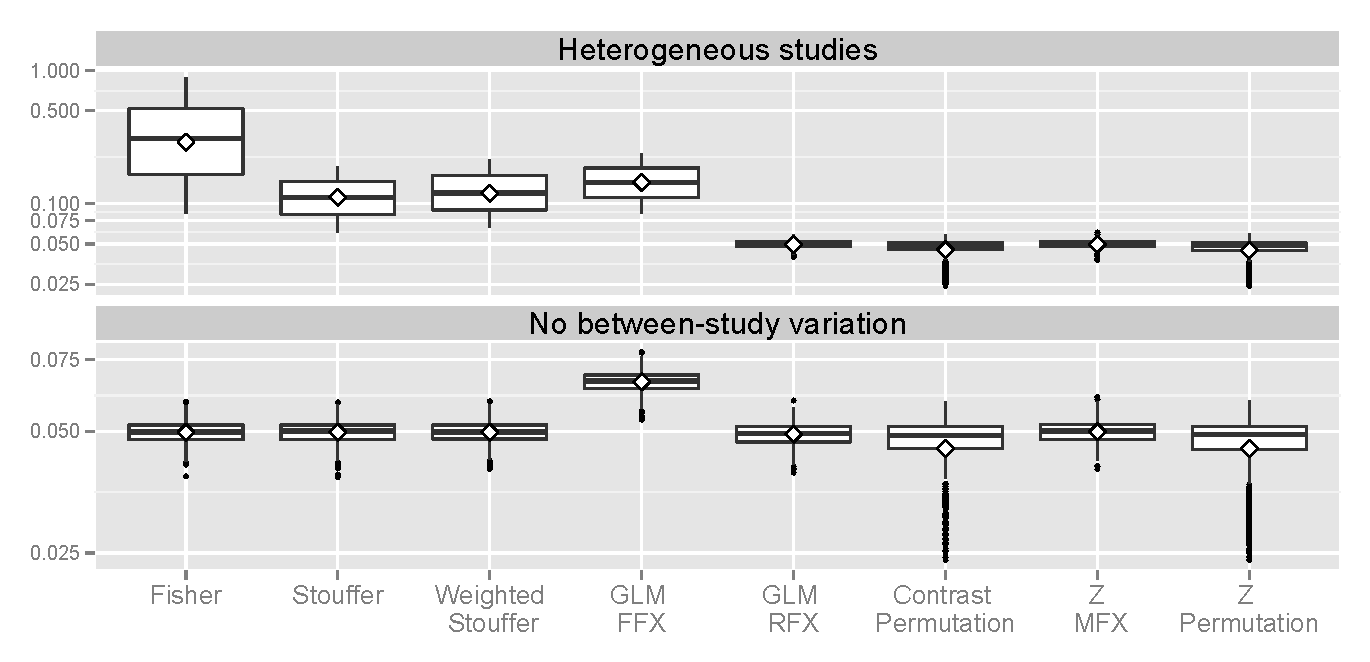
\includegraphics[width=\linewidth]{./MICCAI_version/Rplot_FPR_all.pdf}
	\caption{False positive rates of the meta-analytic estimators under the null hypothesis for $p<0.05$.}
	\label{fig_fpr_all}
\end{figure}

\section{Methods}\label{sec:methods}

% TODO: cite nibabel & other python package (numpy, etc.)
% TODO: say how we computed the CI for the qqplots
% TODO: add links to GitHub repo
% TODO: table FFX GLM should sum up to k x n
% TODO: Stouffers RFX needs to be understood better to state assumptions and revisit results

\subsection{Theory}
For study $\studyidx=1,\ldots,\nStudies$ we have contrast estimate $\effect$, its contrast variance estimate $\vareffect$ (i.e. squared standard error), its equivalent Z-statistic map $Z_i$ and its sample size $n_i$.  

\paragraph{Combining contrast estimates and their standard error}

The recommanded approach is to fit contrast estimates and their standard error with a hierarchical general linear model (GLM)~\cite{Cummings2004}, creating a third-level (level ~1:~subject; level~2:~study; level~3:~meta-analysis). The general formulation for the study-level data is a meta-regression:

\begin{equation}
	\vec{\effectvector} = X \metaanalyticeffects + \epsilon
	\label{eq_meta_GLM}
\end{equation}
where $\vec{\effectvector} = [\effect[1] \ldots \effect[\nStudies] ]\transpose$ is the vector of contrast estimates, $X$ is the $\nStudies \times \nMetaAnalyticEffects$ study-level matrix. While the design matrix $X$ can take any form, typically a one-sample model is used with $\nMetaAnalyticEffects==1$ and $X$ comprised of a column of ones. $\metaanalyticeffects  = [\metaanalyticeffect[1] \ldots \metaanalyticeffect[\nMetaAnalyticEffects] ]\transpose$ is a vector of meta-analytic parameters to estimate and $\epsilon \sim \mathcal{N}(0,W)$ is the residual error term. 

In the most general case of a random-effects meta-analysis, i.e. assuming non-zero between-study variance, we have $W = \mathrm{diag}( \varWithinCon[1] + \varBetween, \ldots ,\varWithinCon[\nStudies] + \varBetween )$ where $\varBetween$ denotes the between-study variance and $\varWithinCon$ denotes the variance of the contrast estimate for study $i$. Eq.~\eqref{eq_meta_GLM} can be solved by weighted least squares giving:

\begin{eqnarray}
	\vec{\hat \metaanalyticeffects}  &=& (X\transpose W^{-1} X)^{-1} X\transpose W^{-1} \vec{\effectvector} \\
	\Var(\vec{\hat \metaanalyticeffects})  &=& (X\transpose W^{-1} X)^{-1}
	\label{eq_WLS}
\end{eqnarray}

Table~\ref{table:estimates_wls_test1} and \ref{table:estimates_wls_test2} provides the WLS estimates and their sampling variances for one and two-sample tests. But in practice, the weight matrix $W$ is unknown and has to be estimated from the data. Given $\hat W$ a consistent estimate of $W$, the feasible generalized least squares (FGLS) estimator is computed as:
\begin{eqnarray}
	\vec{\hat \metaanalyticeffects}  &=& (X\transpose \hat{W}^{-1} X)^{-1} X\transpose \hat{W}^{-1} \vec{\effectvector} \\
	\Var(\vec{\hat \metaanalyticeffects})  &=& (X\transpose \hat{W}^{-1} X)^{-1}
	\label{eq_FGLS}
\end{eqnarray}

Here we use $\vareffect$ as an estimate of $\varWithinCon$ and estimate $\estvarBetween$ from the data. FGLS is asymptotically efficient but its finite sample properties are unknown~\cite{Greene2012}. We used the `FLAME~1' implementation available in FSL that provides inference by comparing the statistic to a Student distribution with $\nStudies-\nMetaAnalyticEffects$ degrees of freedom~\cite{Woolrich2004} as depicted in Table~\ref{table:stats_test1}. This reference approach will be referred to as \textbf{Mixed-effects (MFX) GLM}.

% TODO: is there a better ref for FFX dof than FEAT user manual?
In a fixed-effects meta-analysis, i.e. assuming no or negligible between-study variance, we have $W = \mathrm{diag}( \varWithinCon[1], \ldots ,\varWithinCon[\nStudies])$. We obtain a feasible generalied least squares estimate by approximating $\varWithinCon$ by $\vareffect$. We used the `Simple OLS' implementation available in FSL that provides inference by comparing the statistic to a Student distribution with $(\sum_{i=1}^\nStudies (\nSubjects - 1)) -\nMetaAnalyticEffects$ degrees of freedom~\cite{FEATUserGuide} as depicted in Table~\ref{table:stats_test1}. This reference approach will be referred to as \textbf{Fixed-effects (FFX) GLM}.

% TODO: Review assumptions for RFX Z & Z Perm

\begin{table*}[t]
\begin{center}
\setlength{\tabcolsep}{3pt}
\begin{tabular}{cccccl}
				& Meta-analysic statistic			& Nominal H$_0$ distrib. & Inputs &  Assumptions\\
\hline						
MFX GLM 		& $ \left( \sum \kappa_i \effect \right) / \sqrt{\sum_{i=1}^\nStudies \kappa_i}$ with $\kappa_i = 1/(\estvarBetween + \vareffect)$ & $\mathcal{T}_{\nStudies - 1}$ & $\effect, \vareffect$& IGE, large sample.\\
RFX GLM 		& $  \left( \sum_{i=1}^\nStudies \frac{\effect}{\sqrt{\nStudies} } \right) / \widehat\varCombined  $ & $\mathcal{T}_{\nStudies - 1}$ & $\effect$ & IGE; $\varBetween+\varWithin = \varCombined\; \forall i$ \\
Contrast Perm.	& $ \left( \sum_{i=1}^\nStudies \frac{\effect}{\sqrt{\nStudies}} \right) /\widehat\varCombined  $ & Empirical & $\effect$ & ISE.\\
FFX GLM 		& $  \left(  \sum_{i=1}^{\nStudies}  \frac{\effect}{\vareffect} \right) / \sqrt{\sum_{i=1}^\nStudies 1/\vareffect } $ & $\mathcal{T}_{ (\sum_{i=1}^\nStudies n_i - 1) - 1}$ & $\effect, \vareffect$ 
& $\varBetween=0$, large sample.\\
Fisher	& $ \displaystyle -2 \sum_{\studyidx} \ln \peffect $ & $\chi^2_{(2\nStudies)}$ & $\zeffect$ & $\varBetween=0$\\
Stouffer& $ \displaystyle \sqrt{\nStudies} \times \frac{1}{\nStudies} \sum_{\studyidx} \zeffect $ & $\mathcal{N}(0,1)$ & $\zeffect$& $\varBetween=0$\\
Weighted Z& $  \displaystyle \frac{1}{\sqrt{\sum_{\studyidx} n_\studyidx}} \sum_{\studyidx}  \sqrt{n_\studyidx} \zeffect  $ & $\mathcal{N}(0,1)$ & $\zeffect, \nSubjects$ & $\varBetween=0$\\
Z RFX& $ \left(   \sum_{i=1}^\nStudies \zeffect \right)/ \sqrt{\nStudies} \hat \sigma$ & $\mathcal{T}_{\nStudies-1}$ & $\zeffect$& IGE; $1 + \varBetween/\varWithin$ cst.\\
Z Perm.	& $\left(  \sum_{i=1}^\nStudies \zeffect \right) / \sqrt{\nStudies}$ & Empirical & $\zeffect$ & ISE.\\
\hline 

\end{tabular}
\end{center}
\caption{Statistics for one-sample meta-analysis tests and their sampling distributions under the null hypothesis $H_0$. Empirical null distributions are determined using permutations with sign flipping. \IGE=Independent Gaussian Errors, \ISE=Independent Symmetric Errors. Note: $\peffect = \Phi(-\zeffect)$, $\widehat\varCombined$ is the unbiased sample variance.}
\label{table:stats_test1}
\end{table*}	

\paragraph{Combining contrast estimates}
If the $\vareffect$ are unavailable, the contrast estimates $\effect$ can be combined by assuming that the within-study contrast variance $\varWithinCon$ is constant ($\varWithinCon = \sigma^2 \;\; \forall i$) or negligible in comparison to the between-study variance ($\varWithinCon \ll \varBetween$). Then $W = \mathrm{diag}( \varCombined, \ldots, \varCombined )$ where $\varCombined$ combines the within and between-study variances, i.e.\ $\varCombined \simeq \varBetween$ or $\varCombined \simeq \varBetween + \varWithinCommon$ (note, however, in this setting we do not separately estimate $\varBetween$ or $\varWithinCommon$). Under these assumptions, Eq.~\eqref{eq_meta_GLM} can be solved by ordinary least squares giving:

\begin{eqnarray}
	\hat \metaanalyticeffects  &=& (X\transpose X)^{-1} X\transpose \effectvector \\
	\Var(\hat \metaanalyticeffects)  &=& (X\transpose X)^{-1} \varCombined
	\label{eq_OLS}
\end{eqnarray}

Given $\estvarCombined$ the unbiased sample variance, we obtain the statistics presented in Table~\ref{table:stats_test1} for one sample tests. This approach will be referred to \textbf{Random-effects (RFX) GLM} in the following. Inference can be carried out by comparing the RFX GLM statistic to a Student distribution with $\nStudies-1$ degrees of freedom, this result holds asymptotically as well as in small samples~\cite{Greene2012}. 

As an alternative to parametric approaches, non-parametric inference~\cite{Holmes1996,Nichols2002} can be performed by comparing the one-sample RFX GLM T-statistic to the distribution obtained with ``sign flipping'', i.e.\ randomly multiplying each study's data by 1 or -1, justified by an assumption of independent studies and symmetrically distributed random error. For two-sample tests, the non-parameteric distribution can be obtained by random permutation of the group labels. This approach will be referred to as \textbf{Contrast permutation}.

\paragraph{Combining standardised statistics} 
When only test statistic images are available there are a several alternative approaches available. \textbf{Fisher}'s meta-analysis provide a statistic to combine the associated p-values~\cite{Fisher1932}. \textbf{Stouffer}'s approach combines directly the standardised statistic~\cite{Stouffer1949}. In \cite{Zaykin2011} following \cite{Liptak1958}, the author proposed a weighted method that weights each study's $\zeffect$ by the square root of its sample size [3,7]. This approach will be referred to as \textbf{Weighted Z}. All these meta-analytic statistics assumes no or negligible between-study variance and are only suited for one-sample tests. The corresponding statistics and nominal null distributions are presented in Table~\ref{table:stats_test1}.

As suggested in~\cite{Salimi-khorshidi2009}, to get an RFX-like method based on Stouffer's approach, the standardised statistical estimates $\zeffect$ can be combined in an OLS analysis. The corresponding estimate, referred as \textbf{Z RFX} is also provided in~\ref{table:stats_test1}. 
Non-parametric inference~\cite{Holmes1996,Nichols2002} can also be obtained by sign flipping on the $\zeffect$'s. This approach will be referred to as \textbf{Z permutation}.

\subsection{Approximations}  In practice, all the methods are either approximate in small samples or rely on assumptions that might not be verified in the context of neuroimaging meta-analyses. Methods based on FGLS (MFX GLM and FFX GLM) have approximate parametric null distributions. The nominal distributions of RFX GLM and two-sample contrast permutations are under the (unrealistic) assumption of homogeneous standard errors over studies; even if all studies are `clean' and conducted at the same center, variation in sample size will induce differences in $\vareffect$'s. The fixed-effects methods (Fisher, Stouffer, wieghted Z and FFX GLM) assume homogeneity across studies, i.e. zero between-study variance. All contrast methods (MFX GLM, RFX GLM, Contrast permutation and FFX GLM) require the contrasts to be expressed with in the same units. Finally, RFX Stouffer and Z RFX are ad-hoc methods and their validity has to be investigated.

% \begin{figure}[t]
% 	\centering
% 	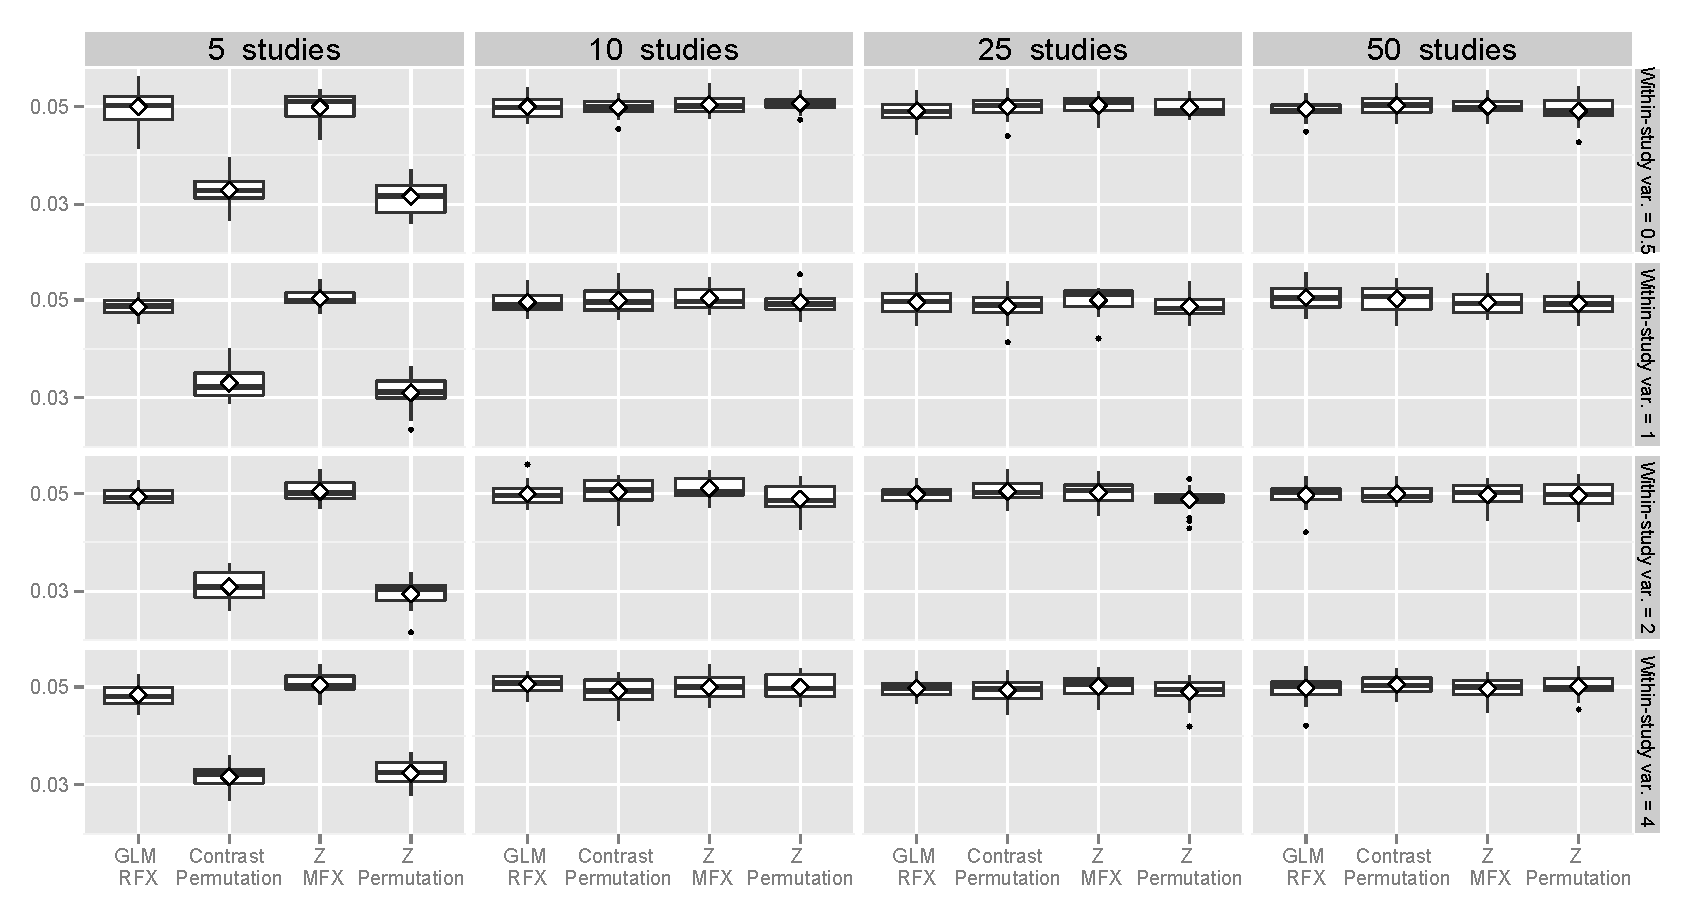
\includegraphics[width=\linewidth]{./MICCAI_version/Rplot_valids.pdf}
% 	\caption{False positive rates of the RFX meta-analytic estimators under $H_0$ for $p<0.05$ as a function of the number of studies and the within-study variance.}
% 	\label{fig_fpr_valid}
% \end{figure}

\subsection{Experiments}

\subsubsection{Validity on null data}
We used Monte Carlo simulations to empirically investigate the validity of each estimator. We simulated a set of  contrast estimates $\effect$ and contrast variance estimates $\vareffect$ according to:
\begin{eqnarray}
	\effect &\sim& \mathcal{N}(0, \frac{\varWithin}{\nSubjects[]}+\varBetween) \\
	\vareffect &\sim& \frac{\varWithin}{\nSubjects[]}  \frac{\chi^2_{(\nSubjects[]-1)}}{\nSubjects[]-1} %
\end{eqnarray}
where $\varWithin$ was either constant across studies (homoscedasticity) and taken from $\{\nSubjects[] \times [0.25, 0.5, 1, 2, 4] \}$ or varying across studies (heteroscedasticity) such as $\max(\varWithin) = \alpha \min(\varWithin)$ with $\alpha \in \{2, 4, 8, 16\}$ and $\text{mean}(\varWithin) = 1$, allowing for 5 different values of $\varWithin$ that were linearly spaced and repeated as many times as needed for the specified number of studies $\nStudies$. The between-study variance $\varBetween$ was set to zero (homogeneity) or $1$ (heterogeneity). We looked at four different number of studies per meta-analysis $\nStudies \in \{5, 10, 25, 50\}$ and two number of subjects $\nSubjects[] \in \{20, 100\}$. We set the default number of subjects per studies to $\nSubjects[]=20$ which is a common sample size in existing neuroimaging studies~\cite{Poldrack2017}. A total of 144 parameter sets ($9 \varWithin \times 2 \varBetween \times 4 \nStudies \times 2 \nSubjects$) was therefore tested and a total of $1~026~000$ realisations was performed for each parameter set.

Three types of analyses were computed: a one-sample meta-analysis testing significance of the mean effect in a group of \nStudies studies, a two-sample meta-analysis testing significance in mean differences between two groups of $\nStudies$ studies each and an unbalanced two-sample meta-analysis testing significance in mean differences between two groups of $2/5 \times \nStudies$ and $8/5 \times \nStudies$ respectively. Two-sample analysis asuumed a common between-study variance across groups.

We conducted those simulations to evaluate the validity of each estimator in small samples and under violations of their assumptions, such as inhomogeneity of contrast variances $\vareffect$ or presence of non-negligible between-study variance. Furthermore, we studied the robustness of contrast-based methods to the presence of mismatched units across studies. To simulate units mismatch, each contrast estimates $\effect$ and contrast variance estimates $\vareffect$ was replaced by a rescaled version: $\effectunits = \effect a_i$ and $\vareffectunits = \vareffect a_i^2$. 2 types of unit mismatched were investigated: 
\begin{itemize}
	\item Mismatched contrast vectors: $a_i$ linearly sampled between $0.4$ and $1.6$ (mean 1).
	\item Mismatched data scaling algorithms (simulating data from different analysis sofware): either 20\% or 50\% of the studies were rescaled with a factor $a_i = 2$ other studies keeping the original scaling.
\end{itemize}
In the case of two-sample tests, the same mismatch was applied to both groups.

% TODO: add version of IBMA toolbox and SnPM on zenodo
% TODO add requirements.txt with conda env? Add conda in citations?
% TODO add Matlab citation as 'MATLAB and Statistics Toolbox Release 2012b, The MathWorks, Inc., Natick, Massachusetts, United States.' > http://www.walkingrandomly.com/?p=4767

The simulations were implemented in Matlab R2016b~\cite{release2016bmathworks} on a High Permformance Computing cluster. Code is available at: \url{https://github.com/cmaumet/zmeta_buster} and depends on the IBMA toolbox~cb5aee~\cite{Maumet2014}, SPM12~revision~6196 (RRID:SCR\_007037)~\cite{Friston2007}, FSL~5.0.10 (RRID:SCR\_002823)~\cite{Jenkinson2012} and SnPM~f254ff (RRID:SCR\_002092)~\cite{Nichols2002}. Figures were computed in R~\cite{RCoreTeam2016} jupyter notebooks~\cite{Perez2007} and depends on ggplot2~\cite{Hadley2009} and cowplot~\cite{Wilke2016}. The code used to compute the figures displayed in this manuscript is available at: \url{https://github.com/cmaumet/zmeta}.

% TODO: table summarising the simulations
% The full set of simulations is summarised is table~\ref{table:simu_settings}. 

\subsubsection{Accuracy on real data}
We then used Receiver-Operating-Characteristics (ROC) curves to assess the sensibility of each of the nine meta-analytic estimators on real data. We used a dataset of 21 studies investigating pain of which 10 were computed with SPM and 11 with FSL, this dataset is available at: http://neurovault.org/collections/1425/. 

% TODO add ref to nidmres library 

Comparability of contrast estimates depends on equivalent scaling of the data, models, and contrast vectors. Data scaling in FSL is performed by setting the median brain intensity to 10,000 while in SPM the mean brain intensity is set to 100. Furthermore, due to imprections of SPM data scaling algorithm, gray matter values tends to be closer to 200 than 100. We therefore resclaled SPM contrast estimates and standard errors by 2 and FSL contrast estimates and standard errors by 100. Furthermore when contrasts were not constructed to preserve units, with sum of positive elements equal to 1, sum of negative elements equal to -1, we further rescale the data to take into account these undesired effects.

We used Neurosynth~\cite{Yarkoni2011}'s automated large scale coordinate-based meta-analysis of pain as ground truth of areas that should present an effect (cf. http://neurosynth.org/analyses/terms/pain/). For each meta-analytic approach, we estimated the true positive rate over a range of thresholds and combined these values to the false positive rates computed on simulated data to create the ROC curves. 

The real data analyses were implemented in Matlab R2016b on a Mac Book Pro laptop. Code is available at: \url{https://github.com/cmaumet/zmeta_rocs}. Software dependencies and repositories for figures are identical as for simulated analyses. Real data figures were computed in Python 3.6.0~\cite{van1995python} jupyter notebooks and depends on nibabel~\cite{Brett2016}, Scipy~\cite{Scipy2001}, numpy~\cite{walt2011numpy}, scikit-learn~\cite{pedregosa2011scikit} and matplotlib~\cite{hunter2007matplotlib}.


\subsubsection{Presence of heterogeneity and heteroscedasticity in real data}
% TODO Add the original citation to Cochran's Q test, read and possibily cite "DETECTING AND DESCRIBING HETEROGENEITY IN META-ANALYSIS REBECCA J. HARDY * AND SIMON G. THOMPSON MRC"
% TODO check the hetergogenity paper to see if we should compute other stats (H?) as well?

To investigate the presence of between-study variations we used Cochran's Q test of heterogeneity~\cite{higgins2002quantifying}:

\begin{equation}
	Q = \sum_{i=1}^{i=k} w_i (\hat \beta_i - \hat \theta)^2
\end{equation}
where $\hat \theta$ is the fixed-effects GLM meta-analytic estimate such that $\hat \theta = \frac{\sum_{i=1}^{i=k}  w_i \hat \beta_i}{\sum_{i=1}^{i=k}  w_i}$. The theoretical weights are $w_i = n_i/\sigma^2_i$, but in practice we use $w_i = 1/s_i^2$. The nominal null distribution of $Q$ is $\chi^2_{\nStudies-1}$

We also computed the $I^2$ statistics:
% "Quantifying heterogeneity in a meta-analysis Julian" gives a different I^2 than the one we used, we should have another look as it is really close to what we have for heterogeneity vs heteroscedasticity.
\begin{equation}
	I^2 = \frac{\estvarBetween}{\estvarBetween + \hat \sigma^2}
\end{equation}

We used the between-study variance estimated by FSL's FLAME~\cite{Smith2001} and computed $\hat \sigma^2$ was computed as the average within-study contrast variance across all studies. Using this metric, voxels with values close to 0 present negligible between-study variance and values close to 1 outline appreciable study heterogeneity and the importance of random-effects models.


\section{Results}\label{sec:results}

\subsection{Robustness to violation of model assumptions}

\begin{figure}[h]
	\centering
 	\includegraphics[trim={0 0 0 0
 	},clip,width=0.8\linewidth]{../../../../Softs/zmeta/small_samples/robustness.pdf}
	\caption{Deviation from theoretical P-values in one-sample tests under violations of the underlying model assumptions: small sample sizes~(A), heteroscedasticity~(B) and heterogeneity~(C). P-values are displayed using a negative log$_{10}$ scale.}
	\label{fig:robustness}
\end{figure}

% TODO: lengend needs to be reworeked: in particular rework "factor(withinInfo)" 

% \begin{figure}[h]
% 	\centering
%  	\includegraphics[width=0.8\linewidth]{../../../../Softs/zmeta/small_samples/test1_smallsample_robustness_subjects_p.pdf}
% 	\caption{Deviation from theoretical P-values in one-sample tests under ideal circunstances with respect to heterogeneity for each statistical approach ($\varBetween=0$ for FFX and $\varBetween=1$ for MFX) and $\nSubjects = 20, 100$ with matched (``nominal'') units.}
% 	\label{small_number_of_subjects_test1}
% \end{figure}

Fig.~\ref{fig:robustness}A presents the one-sample simulation results in small samples, i.e. under small number of studies or small number of subjects. We focus here on methods fow which valitidy is only guaranteed in large samples: FFX GLM and MFX GLM, under ideal conditions otherwise (i.e. $\varBetween$=0 for FFX GLM and $\varBetween$=1 for MFX GLM). When the number of subjects is small, FFX GLM is invalid for all within-study variances investigated, regardless of the number of studies included in the meta-analysis. On the other hand MFX GLM is conservative for small number of studies and constant within-study variance. More surprinsingly, while MFX GLM is valid for constant within-study variances it is invalid in the presence of large variations in the within-study variances, regardless of the number of subjects included in each study. 

% TODO: check if I want to keep any of these paragraphs
% In the nominal case, i.e. when the units are matched across studies and contrasts, RFX GLM and Contrast Permutation are valid, as expected. For small P-values, Contrast Permutation is conservative as expected due to the discrete nature of its distribution. In the presence of a high within-study variance, MFX GLM also appears to be conservative. RFX GLM displays the best behaviour with a pattern that is within the 95\% confidence interval of the theoretical Z for all within-study variance studied and only slightly conservative when the within-study variances are varying across studies.

% For small number of studies, permutation methods (including Contrast Permutation and Z permutation) are conservative as expected due to the discrete nature of their distribution (cf. supplementary figure TODO).

% Other approaches (TODO) have a nominal behaviour under small sample sizes as expected according to theory. Only Stouffers MFX presents some invalidity, which can be explained by the fact that this is an had hoc not recommended statistic (cf. supplementary figure TODO).

Fig.~\ref{fig:robustness}B presents the one-sample simulation results under heteroscedasticity ($\varWithin$ varying across studies). We focus here on methods fow which valitidy is only guaranteed under homoscedasticity: RFX and Contrast permutation, in a sample of $25$ studies with $20$ subjects each under ideal conditions otherwise (i.e. $\varBetween$=1). RFX GLM and contrast permutation are robust to heteroscedasticity for all settings studied. RFX GLM is closer to nominal. For small P-values, Contrast Permutation is conservative as expected due to the discrete nature of its distribution.

Fig.~\ref{fig:robustness}C presents the one-sample simulation results under heterogeneity ($\varBetween>0$). We focus here on methods fow which valitidy is only guaranteed under homogeneity: Fisher, Stouffer, Weighted Z and FFX GLM, with a sample of $\nStudies=25$ studies with $\nSubjects=20$ subjects each. All fixed-effects methods are invalid under heterogeneity.

Similar behaviours are observed for two-sample tests (cf. Supplementary Fig.~\ref{fig:robustness_test2} and Fig.~\ref{fig:robustness_test3}).

\subsection{Robustness to units mismatch}

\begin{figure}[h]
	\centering
 	\includegraphics[trim={0 0 0 0
 	},clip,width=0.8\linewidth]{../../../../Softs/zmeta/units_mismatch/units.pdf}
	\caption{Deviation from theoretical P-values in one-sample tests under violations of the underlying model assumptions: small sample sizes~(A), heteroscedasticity~(B) and heterogeneity~(C). Deviation from theoretical Z in two-sample tests with unit mismatch, under ideal circunstances for each statistical approach ($\varBetween=1$ and $\nStudies = 5, 25, 50$ with matched (``nominal'') or mismatched (``different scaling target", ``different scaling algorithm", ``different contrast vector scaling") units.}
	\label{fig:units}
\end{figure}

Fig.~\ref{fig:units} presents the simulation results under unit mismatches for one-sample tests. When different scaling algorithm are used (Fig.~\ref{fig:units}, 2nd and 3rd columns), e.g. with different neuroimaging software packages (provided that differences in scaling targets have been accounted for), Contrast Permutation has a behaviour that is close to nominal. RFX GLM is valid but conservative. MFX GLM is robust to the presence of unit mimatches when the studies are homoscedastic. In the presence of strong heteroscedasticity, MFX GLM remains invalid as when the units are matched due to finite sample inaccuracies (cf. previous section). In the presence of slight heteroscedasticity, unit mismatchs can cause invalidity of othewise valid MFX GLM. When the contrast are scaled differently (Fig.~\ref{fig:units}, 4th column), we observe a very similar pattern than for different scaling algorithm. Similar behaviours are observed for two-sample tests (cf. Supplementary Fig.~\ref{fig:units_test2} and Fig.~\ref{fig:units_test3}).

% TODO: Decide if I need to keep any of the paragraphs below
% \subsubsection{Group meta-analysis}

% Fig.~\ref{test1_k25_btw1} presents the simulation results for a one-sample test with $\varBetween=1$ and a sample size $\nStudies = 5, 25, 50$. For the nominal case, i.e. when the units are matched across studies and contrasts, MFX GLM, RFX GLM and Contrast Permutation are all valid, as expected. For small sample sizes ($\nStudies = 5$), MFX GLM and contrast permutation are both very conservative. For large values of Z, Contrast Estimation is conservative as expected due to the discrete nature of its distribution. More suprinsing, in the presence of a high within-study variance, MFX GLM also appears to be conservative. RFX GLM displays the best behaviour with a pattern that is always within the 95\% confidence interval of the theoretical Z.

% % In the extreme case of different scaling target, i.e. when data where scaled to a different mean (100 versus 10 000), Contrast Permutation displays a pattern that is very close to its nominal behaviour, namely it is valid but conservative for large Z. GLM RFX is valid for Z values that are greater than 1.5 (i.e. the area we are interested in in terms of detections) but very conservative, especially when the number of samples from each scaling factor are not equal. This behaviour is expected as the estimated between-study variance is inflated by the difference in scaling target. MFX GLM is invalid for small within-study variances and conservative for large within-subject variances.


% \subsubsection{Balanced between-group meta-analysis}

% Fig.~TODO presents the simulation results for a two-sample meta-analyses with $\varBetween=1$ and a sample size $\nStudies = 25$. For the nominal case, GLM RFX, GLM RFX and contrast estimation provide valid estimates. Contrast Permutation is conservative for large Z values. Both RFX GLM and MFX GLM display the best behaviour with a pattern that is within the 95\% confidence interval of the theoretical Z.

% In the extreme case of different scaling target, contrast permutation is always valid with a pattern very similar than its nominal behaviour. GLM RFX is valid for Z values greater than 1.5, which is the area of interest in detections, but display a strong conservativness, more pronounced than the Contarst Permutation. GLM MFX is slighlty invalid for all within-study variances except the largest one when 20\% of the studies come from the second software.


% \subsubsection{Unbalanced between-group meta-analysis}


% Fig.~TODO presents the simulation results for unbalanced two-sample meta-analyses with $\varBetween=1$ and a sample size $\nStudies = 25$. For the nominal case, MFX GLM, GLM RFX and contrast permutation provide valide estimate. As expected due to the discrete nature of its ampling distribution, contrast permutation is conservative for large Z value. GLM RFX is conservative. RFX GLM is closest to the theoretical behaviour with Z-values that are always within the 95\% confidence interval.

% In the extreme case of different scaling target, MFX GLM is always valid but slightly conservative. RFX GLM is valid for Z values greater than 1.5 (area of interest in detections) but conservative. Similarly contrast permutation is invalid for Z smaller than 1.5 and conservative otherwise. This can be explained by the violation of the exchangeability condition.

% When different scaling algorithm are used, (same paragraph as for one-sample test)

% When the contrast are scaled differently, we observe a very similar pattern than for different scaling algorithm with higher varaince of the estimates.


% \subsection{Simulations}
% Fig.~\ref{fig_fpr_all} displays the false positive rate at $p<0.05$ obtained for the nine estimators over all set of parameters in the absence and presence of between-study variation. As expected, the fixed-effects meta-analytic summary statistics, i.e.\ Fisher's, Stouffer's and weighted Stouffer's estimates, are liberal in the presence of study heterogeneity. The original Fisher's approach is the most invalid. More surprising, FFX GLM is also invalid with homogeneous studies. The explanation is over-estimation of degrees-of-freedom (DF); while DF is computed as $(\sum n-1)-1$, under heteroscasdicity (from $\sigma_i$ or $\nSubjects$) it will be much lower~\cite{Satterthwaite}. Z MFX and GLM RFX provide valid estimates, and the permutation estimates are valid but tend to be conservative with greater variation in false positive rates.

% The impact of the number of studies involved in the meta-analysis and of the size of the within-study variance are investigated in Fig.~TODO. Permutation inference is valid but conservative when 5 studies are used; this is because there are only $2^5=32$ possible permutations and thus $1/32=0.03125$ is largest attainable valid P-value. All approaches perform equally as soon as 10 or more studies are included in the meta-analysis. 


\subsection{Accuracy on real data}
\begin{figure}[h]
	\centering
 	\includegraphics[trim={0 0 0 0
 	},clip,width=0.8\linewidth]{../../../../Softs/zmeta/roc.pdf}
	\caption{ROC curves of the meta-analytic estimators where true positive rate were computed using a real data meta-analysis of 21 studies of pain and false positive rates using simulated data under various levels of heterogeneity (A) and hetoroscedasticity (B).}
	\label{fig_realdata}
\end{figure}

% TODO: check RFX curve: do we need more points towards zero??
% TODO: redo with data already available on Neurovault??

Fig.~\ref{fig_realdata}A. displays the ROC curves for all the meta-analytic estimators under varying levels of heterogeneity. As expected, the fixed-effects approaches are the most affected by heterogeneity. Hence, Fisher's method is both the most sensitive method under low heterogeneity and the less sensitive under large heterogeneity. Random-effects approaches are relatively insensitive to the level of heterogeneity. Amongst random-effects approaches the most optimal are Stouffers RFX and Z Permutation that display nearly identical ROC curves, followed by MFX GLM, Contrast Permutation and finally RFX GLM. Differences between MFX GLM and RFX GLM are likely to be non-significant as they both had p-values within the 95\% confidence interval.
% TODO: display CIs for FPR??  

Fig.~\ref{fig_realdata}B. displays the ROC curves for all the meta-analytic estimators under varying levels of heteroscedasticity. Again, the fixed-effects approaches are the most sensitive to heteroscedasticity. This can be explained by the fact that under high heteroscedasticy, some studies will present a low (or high) within-study variance, relatively increasing the between-study variance by comparison to the within-study variance. Amongst the random-effects approaches the most optimal are again Stouffer MFX and Z permutation that display nearly identical ROC curves. 

% Fig.~\ref{fig_realdata} plots the difference between the z-score estimated by each meta-analytic approach against the reference z-score computed with MFX GLM. All FFX statistics provide overly optimistic z-estimate suggesting, again, that study heterogeneity is present in the studied dataset.
% Among the RFX meta-analytic approaches, GLM RFX and contrast permutations provide z-scores estimate that are equal or smaller than the reference. Z permutation provides slightly larger z-scores between 1 and 3 (reference p-values between 0.16 and 0.0013) but is mostly in agreement with the reference z-scores. On the other hand, Z MFX is more liberal than the reference for z-score ranging from 3 to 5 (reference p-values between 0.0013 and 2.9e-07) and more stringent for z-scores smaller than 5.


\subsubsection{Presence of heterogeneity and heteroscedasticity in real data}

\begin{figure}[h]
	\centering
 	\includegraphics[width=0.8\linewidth]{../../../../Softs/zmeta/heterogeneity_Q.pdf}
 	\includegraphics[width=0.8\linewidth]{../../../../Softs/zmeta/heterogeneity_test.pdf}
	\caption{Test of heterogeneity using Cochran's Q test: Q statistic (A) and significant P-values in $-\log_{10}$ at FDR-corrected $P<0.05$.}
	\label{fig:heterogeneity_Q}
\end{figure}

\begin{figure}[h]
	\centering
 	\includegraphics[width=0.8\linewidth]{../../../../Softs/zmeta/heterogeneity_I2_between.pdf}
 	\includegraphics[width=0.8\linewidth]{../../../../Softs/zmeta/heterogeneity_I2_mean_within.pdf}
 	\includegraphics[width=0.8\linewidth]{../../../../Softs/zmeta/heterogeneity_I2.pdf}
	\caption{Estimated between-study variance (A), estimated average within-study contrast variance (B) and ratio of the estimated between study-variance onto total variance (i.e. $I^2$) (C).}
	\label{fig:heterogeneity_I2}
\end{figure}

Fig.~\ref{fig:heterogeneity_Q} presents the results of Cochran's Q test of heterogeneity on real data. Overall, 88\% of the voxels displayed significant heterogeneity at FDR-corrected $P < 0.05$. 
Fig.~\ref{fig:heterogeneity_I2} displays the $I^2$ statistic. 27\% of the voxels presented a larger between-study variance. Both statistics therefore support the presence of study heterogeneity (non negligible between-study variance) in this collection of studies.

\begin{figure}[h]
	\centering
 	\includegraphics[width=0.8\linewidth]{../../../../Softs/zmeta/heteroscedasticity.pdf}
	\caption{Boxplot of the parameter estimates across voxels by studies. For each box, the orange line corresponds to the median
and the top and bottom lines of the black square are the upper and lower quartiles of the distribution. The whiskers cover the data
points that are located up to 1.5 times the inter-quartile distance. Points falling out of the whiskers are not displayed. Studies are sorted from smaller to larger interquartile ranges.}
	\label{fig:heteroscedasticity}
\end{figure}

Fig.~\ref{fig:heteroscedasticity} displays the variability of the study parameter estimate across voxels. This plots supports the presence of heteroscedasticity in this dataset.

\section{Discussions}\label{sec:discussion}    
With the growing availability of summary image data for published neuroimaging studies, image-based meta-analysis becomes feasible. Here, we investigated the validity and accuracy of nine meta-analytic estimators under conditions that are typically observed in fMRI and which might invalidate the underlying assumptions of each method.

As expected, fixed-effects methods were shown to be invalid in the presence of heterogeneity. On the other hand, homoscedastic methods were shown to be robust to heteroscedasticity which is in line with published literature on group fMRI statistics~\cite{Mumford2009}. More surprisingly, MFX GLM was showed to be invalid in the presence of large heteroscedasticity due to its approximations not being accurate in small samples. 

In the presence of mismatched units, GLM RFX appeared conservative, while contrast permutation provided the best behaviour, closest to nominal. 
As confirmed by our real data analysis, we do expect heterogeneity to be present in meta-analytic studies due for instance to variations in the analytic procedure including varying experimental designs, analysis workflows or even due to different imaging instruments. The dataset we used in our real data analysis was created within a single lab and using the same neuroimaging analysis software (FSL), our estimates of heteroscedasticity and heterogeneity are likely to be lower than would be typically observed in a dataset pulling more heterogeneous studies. Similarly, we do expect heteroscedasticity to be present for the same reasons as well as due to varying sample sizes across studies. Finally meta-analysis sample sizes are still relatively small. 

Given the still relatively small sample sizes that can be achieved in IBMA as of today, we recommend using RFX GLM, Contrast Permutation, Stouffers MFX or Z Permutation that do not rely on small sample approximations and are robust to both heterogeneity and heteroscedasticity. Unit mismatch across contrasts is likely to be an issue as, even when statistic maps are shared in support of a publication, it is very rare for it to be accompagnied by metadata describing full details on the analysis. Although z-based meta-analyses are suboptimal~\cite{Cummings2004} until full reporting is routinely done, we suggest to use Z-based methods that are insensitive to units. 

% TODO: do we want to say something about corrected/uncorrected p-values? Our simulated data were based on uncorrected p-values. In neuroimaging meta-analyses, results are more likely to be derived using correction for multiple comparisons. Accuracy of uncorrected p-values is important for FDR (and FWE??) and for clusterwise thresholds. 

Because true areas of activations in real data are unknown, we relied on an external source to compute the ground truth activations: the Neurosynth platform which provides very large-scale automatic coordinate-based meta-analysis of the literature. Because this ground truth was determined using a coordinate-based (and not image-based) meta-analysis, it is very likely to be missing some true activated areas with small effect sizes (that would effectively not pass the threshold at the level of a single study). Our estimated true positive rate are therefore likely to be overestimations. 

% Because simulating realistic activations can be particularly challenging 

Because true areas of no activations in real data are unknown, we relied on simulated data to compute the false positive rates. 
% This has the disadvantage of synthetic data listed above.
We only had a single real dataset for meta-analysis and therefore only computed true positive rates once and combined them with the different false positive rates computed by simulations. In practice the sensibility is very likely to vary under different level of heterogeneity, heteroscedasticity and one would need a larger real dataset to fully investigate sensitivity. The most faithful are the ones that correspond to the settings that are closer to the one observed in the real dataset, i.e. is sigma2/20 ~ 1...16. 

 % which is consistent with our general recommendations stated above.
Finally, in our simulations we investigated heteroscedasticity due to varying within-study variances but not due to varying sample sizes. We do expect the results to be consistent (ignoring the $X^2$ dof) but would have to be double checked.


\section{Conclusion}\label{sec:ccl}
We have compared nine meta-analytic approaches in the context of one-sample test. Through simulations, we found the expected invalidity of fixed-effects approaches in the presence of study heterogeneity, but also of FFX GLM even with no between-study variation. In a real dataset of 21 studies of pain, there was evidence for substantial between-study variation that supports the use of random-effects meta-analytic statistics. When only contrast estimates are available, RFX GLM was valid. When only standardised estimates are available, permutation is the preferred option as the one providing the most faithful results. 


\section{Acknowledgements}
We gratefully acknowledge the use of the pain dataset from the Tracey pain group, FMRIB, Oxford. The majority of this work was conducted while TEN and CM were at the University of Warwick and used the High Performance Computing cluster of the Departement of Statistics, University of Warwick.

%
% ---- Bibliography ----

\section{References}
\bibliographystyle{plain}
\bibliography{ibma}

\beginsupplement

\begin{table*}[h]
\begin{center}
\setlength{\tabcolsep}{3pt}
\begin{tabular}{cccccl}
				& $\hat{\metaanalyticeffect[1]}$ & $\Var(\hat{\metaanalyticeffect[1]})$ \\
\hline						
Random effects 		& $ \left( \sum \eta_i \effect \right) / \left( \sum \eta_i \right)$ with $\eta_i = 1/(\varBetween + \varWithin/\nSubjects)$ & $1/\sum \eta_i$ \\
Fixed effects 		& $ \left( \sum \effect \times \varWithinConInv \right) / \left(\sum \varWithinConInv \right)$ & $1/(\sum \varWithinConInv)$\\
\hline 
\end{tabular}
\end{center}
\caption{One-sample weighted least squares (WLS) estimates and their sampling distributions for random-effects and fixed-effects meta-analyses. The FGLS estimates and assumed sampling distributions are obtained by substituing: $\varBetween \leftarrow \estvarBetween$ and $\varWithin/\nSubjects \leftarrow \vareffect$.}
\label{table:estimates_wls_test1}
\end{table*}

\begin{table*}[h]
\begin{center}
\setlength{\tabcolsep}{3pt}
\begin{tabular}{cccccl}
				& $\hat{\metaanalyticeffect[1]}$ - $\hat{\metaanalyticeffect[2]}$ & $\Var(\hat{\metaanalyticeffect[1]}$ - $\hat{\metaanalyticeffect[2]})$\\
\hline						
Random effects 		& $ \displaystyle \left( \sum_{i \in G_1} \eta_i \effect \right) / \left( \sum_{i \in G_1} \eta_i \right) - \left( \sum_{i \in G_2} \eta_i \effect \right) / \left( \sum_{i \in G_2} \eta_i \right)$ with $\displaystyle \eta_i = 1/\left(\varBetween + \varWithin/\nSubjects\right)$ & $\displaystyle 1/\sum_{i \in G_1} \eta_i + 1/\sum_{i \in G_2} \eta_i$\\
Fixed effects 		& $ \displaystyle \left( \sum_{i \in G_1} \effect \times \varWithinConInv \right) / \left(\sum_{i \in G_1} \varWithinConInv \right) - \left( \sum_{i \in G_2} \effect \times \varWithinConInv \right) / \left(\sum_{i \in G_2} \varWithinConInv \right)$ & $\displaystyle 1/ \left( \sum_{i \in G_1} \varWithinConInv\right) + 1/ \left(\sum_{i \in G_2} \varWithinConInv \right)$\\
\hline 
\end{tabular}
\end{center}
\caption{Two-sample weighted least squares (WLS) estimates and their sampling distributions for random-effects and fixed-effects meta-analyses. The FGLS estimates and assumed sampling distributions are obtained by substituing: $\varBetween \leftarrow \estvarBetween$ and $\varWithin/\nSubjects \leftarrow \vareffect$.}
\label{table:estimates_wls_test2}
\end{table*}


\begin{table*}[h]
\begin{center}
\setlength{\tabcolsep}{3pt}
\begin{tabular}{cccl}
				& $ \hat{\metaanalyticeffect[1]} $			& $\Var(\hat{\metaanalyticeffect[1]})$\\
\hline						
RFX GLM 		& $ \sum \effect/\nStudies $ & $ \varCombined/\nStudies $ \\
Z MFX 		& $ \sum \zeffect/\nStudies $ & $ \varCombined/\nStudies $ \\
\hline 
\end{tabular}
\end{center}
\caption{For the meta-analytic approaches based on Ordinary Least Squares (OLS), one-sample meta-analytic estimates and sampling variances. Note that $\varCombined$ will be different for each row of this table.}
\label{table:estimates_test1}
\end{table*}

% TODO: table OLS for two-sample tests

% \begin{table*}[h]
% \begin{center}
% \setlength{\tabcolsep}{3pt}
% \begin{tabular}{cccl}
% 				& $ \hat{\metaanalyticeffect[1]} $			& $\Var(\hat{\metaanalyticeffect[1]})$\\
% \hline						
% MFX GLM 		& $ \left( \sum \kappa_i \effect \right) / \left( \sum \kappa_i \right)$ with $\kappa_i = 1/(\estvarBetween + \vareffect)$ & $1/\sum \kappa_i$\\
% RFX GLM 		& $ \sum \effect/\nStudies $ & $ \varCombined/\nStudies $ \\
% FFX GLM 		& $ \left( \sum \effect \times \varWithinConInv \right) / \left(\sum \varWithinConInv \right)$ & $1/(\sum \varWithinConInv)$\\
% Contrast Perm.	& $ \sum \effect/\nStudies $\\
% Z MFX 		& $ \sum \zeffect/\nStudies $ & $ \varCombined/\nStudies $ \\
% Z Perm.	& $\left(  \sum_{i=1}^\nStudies \zeffect \right) / \sqrt{\nStudies}$ \\
% \hline 

% \end{tabular}
% \end{center}
% \caption{Two-sample meta-analytic estimates and sampling variance. Note: $\peffect = \Phi(-\zeffect)$}
% \label{table:estimates_test1}
% \end{table*}

\begin{figure}[h]
	\centering
 	\includegraphics[trim={0 0 0 0
 	},clip,width=0.8\linewidth]{../../../../Softs/zmeta/small_samples/robustness_test2.pdf}
	\caption{Deviation from theoretical P-values in two-sample tests under violations of the underlying model assumptions: small sample sizes~(A), heteroscedasticity~(B) and heterogeneity~(C). P-values are displayed using a negative log$_{10}$ scale.}
	\label{fig:robustness_test2}
\end{figure}

\begin{figure}[h]
	\centering
 	\includegraphics[trim={0 0 0 0
 	},clip,width=0.8\linewidth]{../../../../Softs/zmeta/small_samples/robustness_test3.pdf}
	\caption{Deviation from theoretical P-values in unbalanced two-sample tests under violations of the underlying model assumptions: small sample sizes~(A), heteroscedasticity~(B) and heterogeneity~(C). P-values are displayed using a negative log$_{10}$ scale.}
	\label{fig:robustness_test3}
\end{figure}

\begin{figure}[h]
	\centering
 	\includegraphics[trim={0 0 0 0
 	},clip,width=0.8\linewidth]{../../../../Softs/zmeta/units_mismatch/units_test2.pdf}
	\caption{Deviation from theoretical P-values in one-sample tests under violations of the underlying model assumptions: small sample sizes~(A), heteroscedasticity~(B) and heterogeneity~(C). Deviation from theoretical Z in two-sample tests with unit mismatch, under ideal circunstances for each statistical approach ($\varBetween=1$ and $\nStudies = 5, 25, 50$ with matched (``nominal'') or mismatched (``different scaling target", ``different scaling algorithm", ``different contrast vector scaling") units.}
	\label{fig:units_test2}
\end{figure}

\begin{figure}[h]
	\centering
 	\includegraphics[trim={0 0 0 0
 	},clip,width=0.8\linewidth]{../../../../Softs/zmeta/units_mismatch/units_test3.pdf}
	\caption{Deviation from theoretical P-values in one-sample tests under violations of the underlying model assumptions: small sample sizes~(A), heteroscedasticity~(B) and heterogeneity~(C). Deviation from theoretical Z in two-sample tests with unit mismatch, under ideal circunstances for each statistical approach ($\varBetween=1$ and $\nStudies = 5, 25, 50$ with matched (``nominal'') or mismatched (``different scaling target", ``different scaling algorithm", ``different contrast vector scaling") units.}
	\label{fig:units_test3}
\end{figure}



% %
% \begin{thebibliography}{5}
% %
% \bibitem {clar:eke}
% Clarke, F., Ekeland, I.:
% Nonlinear oscillations and
% boundary-value problems for Hamiltonian systems.
% Arch. Rat. Mech. Anal. 78, 315--333 (1982)

% \bibitem {clar:eke:2}
% Clarke, F., Ekeland, I.:
% Solutions p\'{e}riodiques, du
% p\'{e}riode donn\'{e}e, des \'{e}quations hamiltoniennes.
% Note CRAS Paris 287, 1013--1015 (1978)

% \bibitem {mich:tar}
% Michalek, R., Tarantello, G.:
% Subharmonic solutions with prescribed minimal
% period for nonautonomous Hamiltonian systems.
% J. Diff. Eq. 72, 28--55 (1988)

% \bibitem {tar}
% Tarantello, G.:
% Subharmonic solutions for Hamiltonian
% systems via a $\bbbz_{p}$ pseudoindex theory.
% Annali di Matematica Pura (to appear)

% \bibitem {rab}
% Rabinowitz, P.:
% On subharmonic solutions of a Hamiltonian system.
% Comm. Pure Appl. Math. 33, 609--633 (1980)

% \end{thebibliography}


\end{document}

%%
%% End of file `elsarticle-template-1-num.tex'.